\renewcommand{\thefigure}{S\arabic{figure}}
\setcounter{figure}{0}

\section{Appendix - Supplementary Information}

\begin{figure*}[t!]
\begin{center}
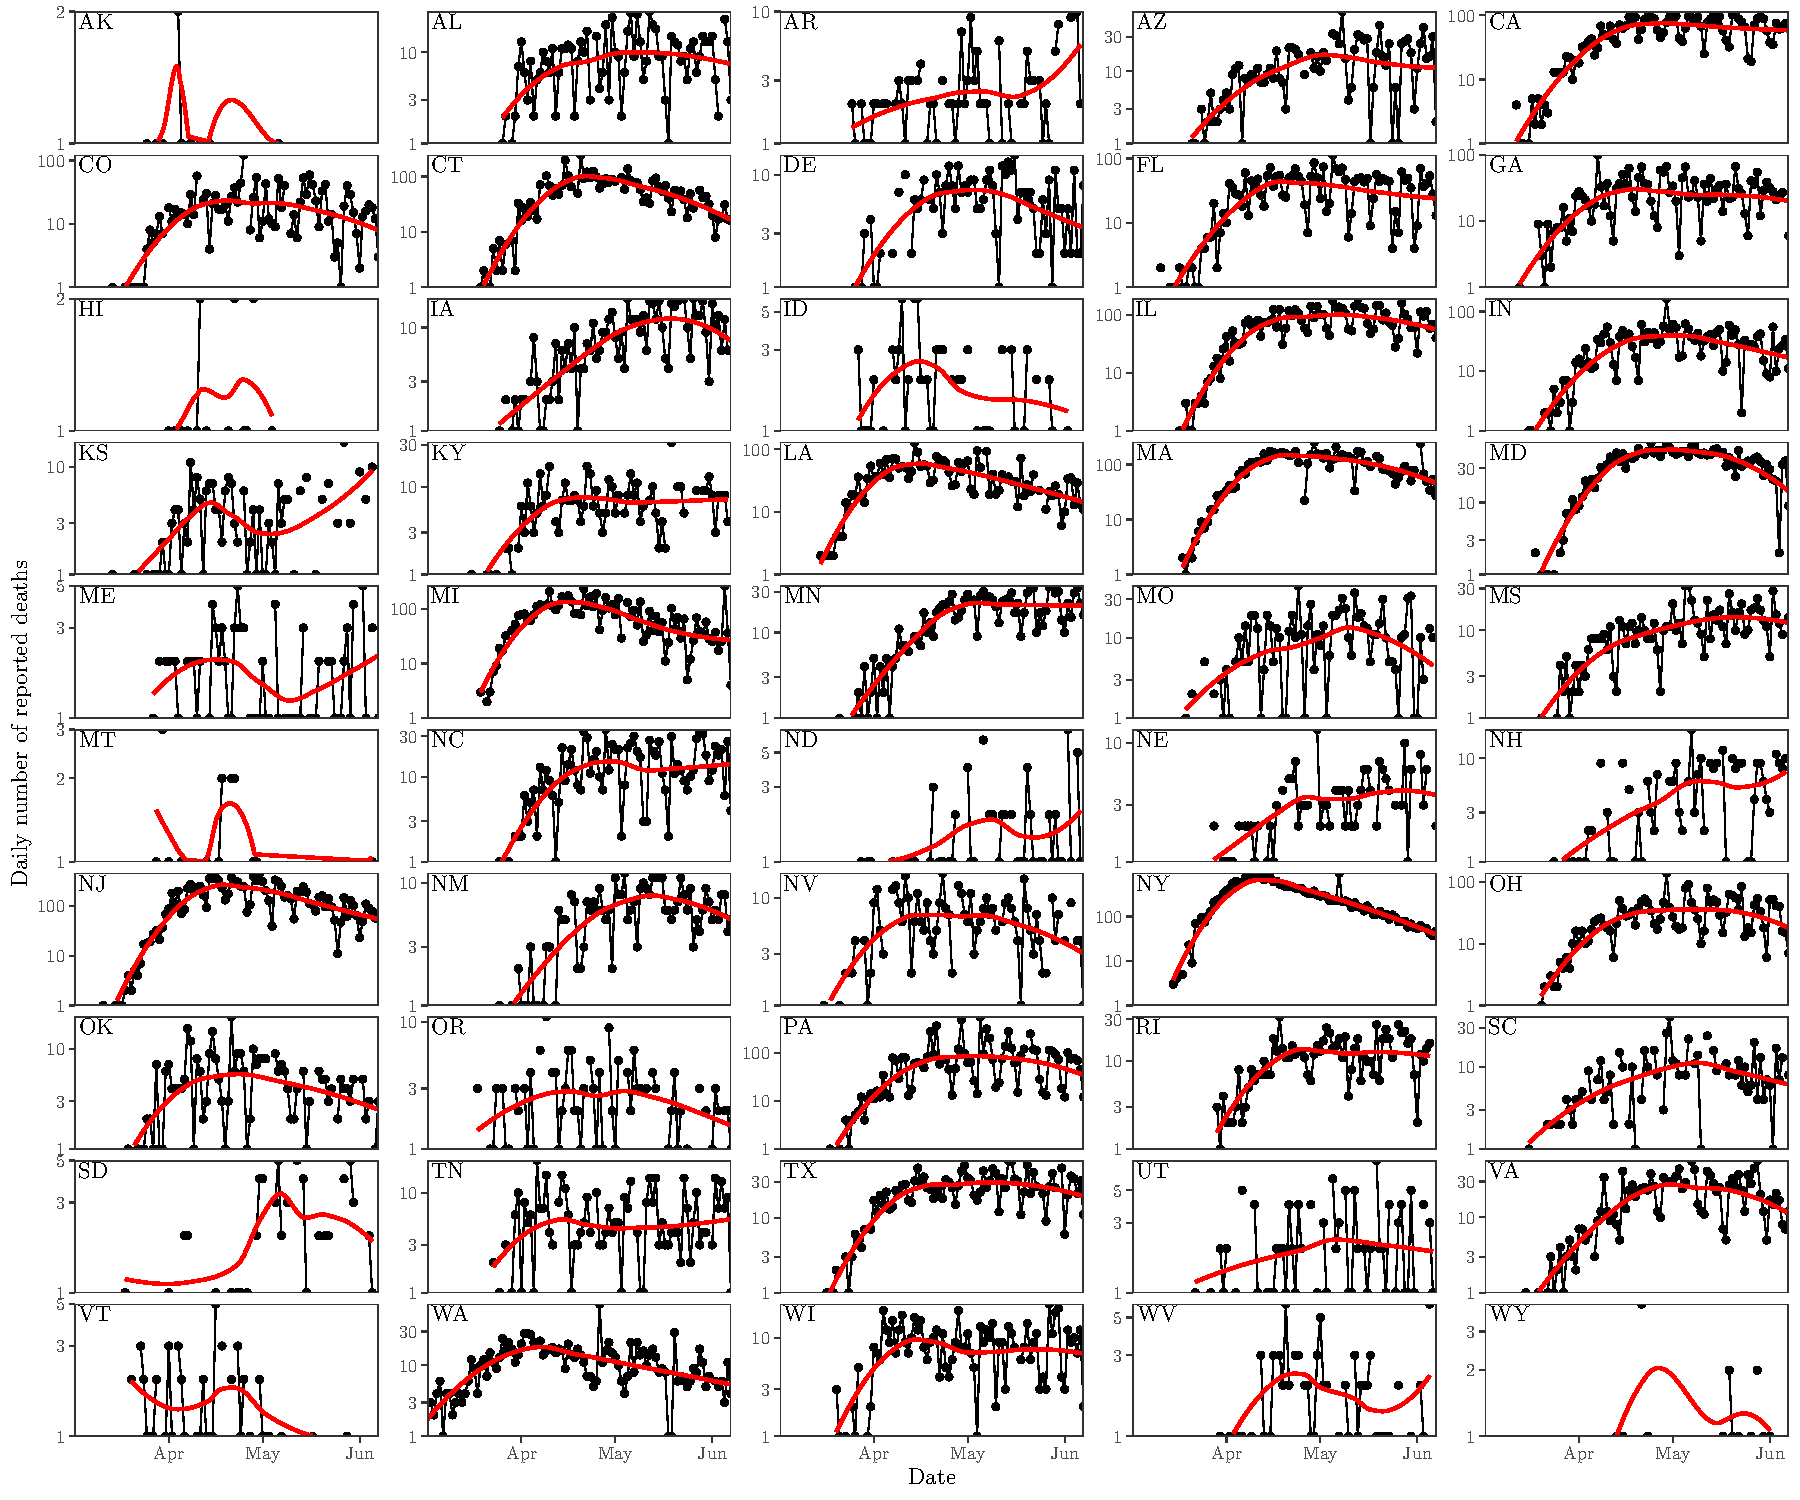
\includegraphics[width=0.45\textwidth]{deaths/deaths.pdf}
\caption{Daily number of reported deaths for COVID-19 (black points and lines) and the corresponding locally estimated scatterplot smoothing (LOESS) curves (red lines) in 50 states.
%Daily number of deaths is smoothed in log space, only including days with one or more reported deaths.
\label{fig.supp_plateaus}}
\end{center}
\end{figure*}

\begin{figure*}[t!]
\begin{center}
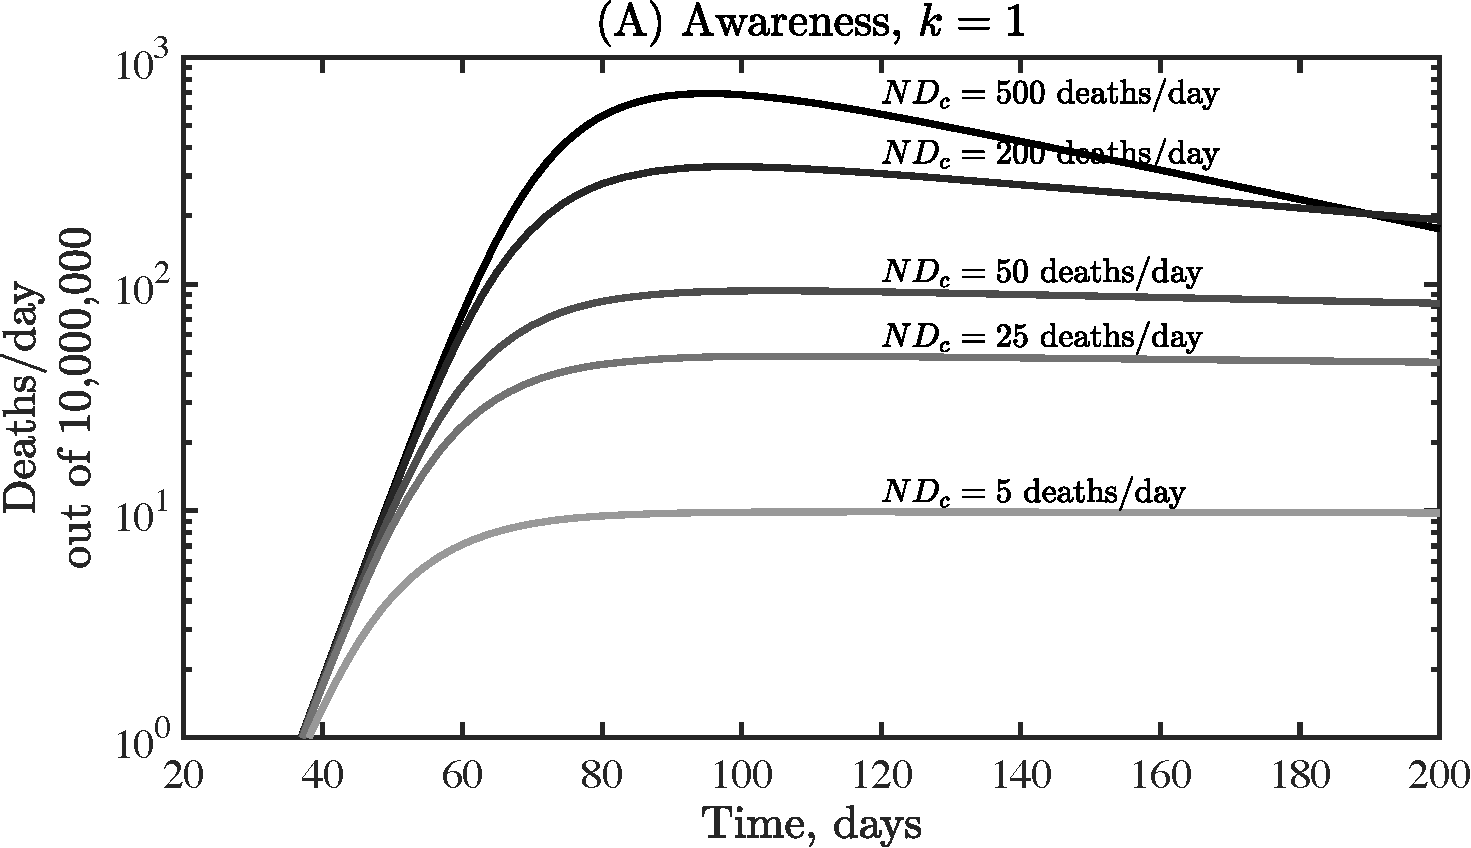
\includegraphics[width=0.4\textwidth]{scripts/figseir_Speak_k1_noname.pdf}
\mbox{\hspace{0.05\textwidth}}
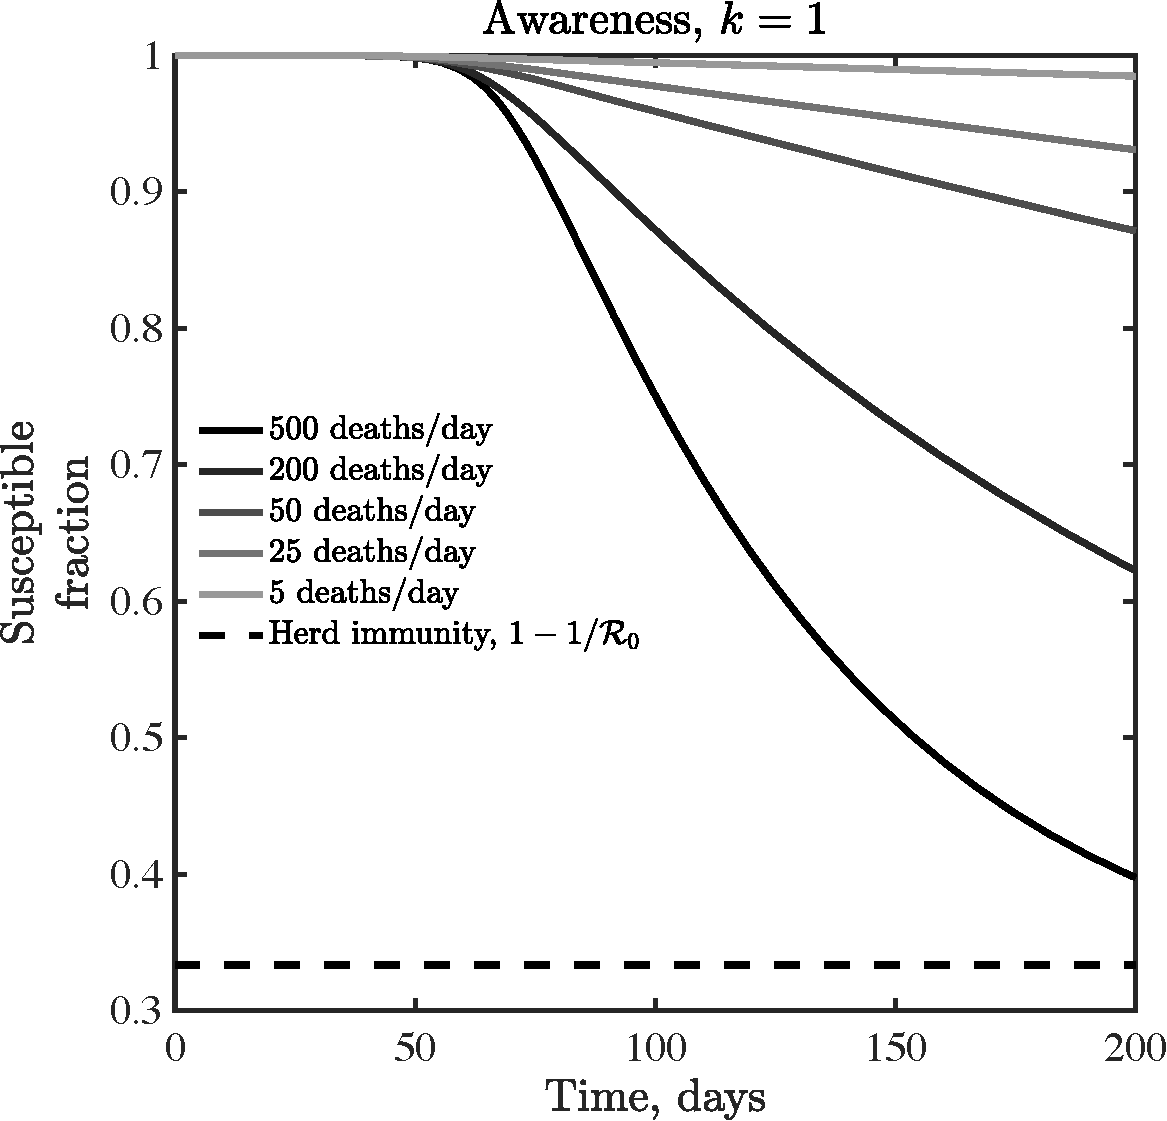
\includegraphics[width=0.4\textwidth]{scripts/figseir_Susc_k1_noname.pdf}\\
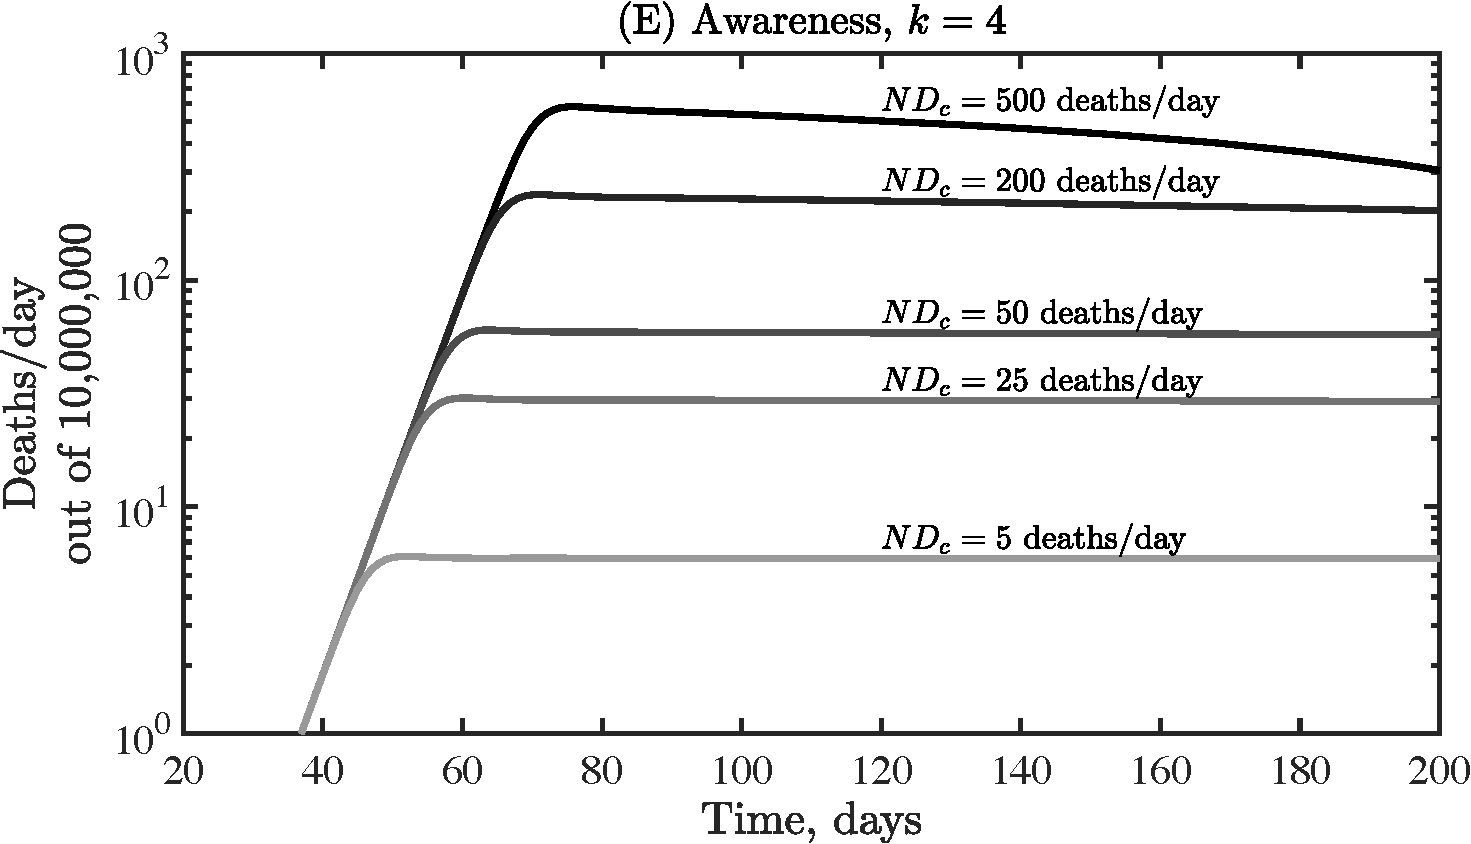
\includegraphics[width=0.4\textwidth]{scripts/figseir_Speak_k4_noname.pdf}
\mbox{\hspace{0.05\textwidth}}
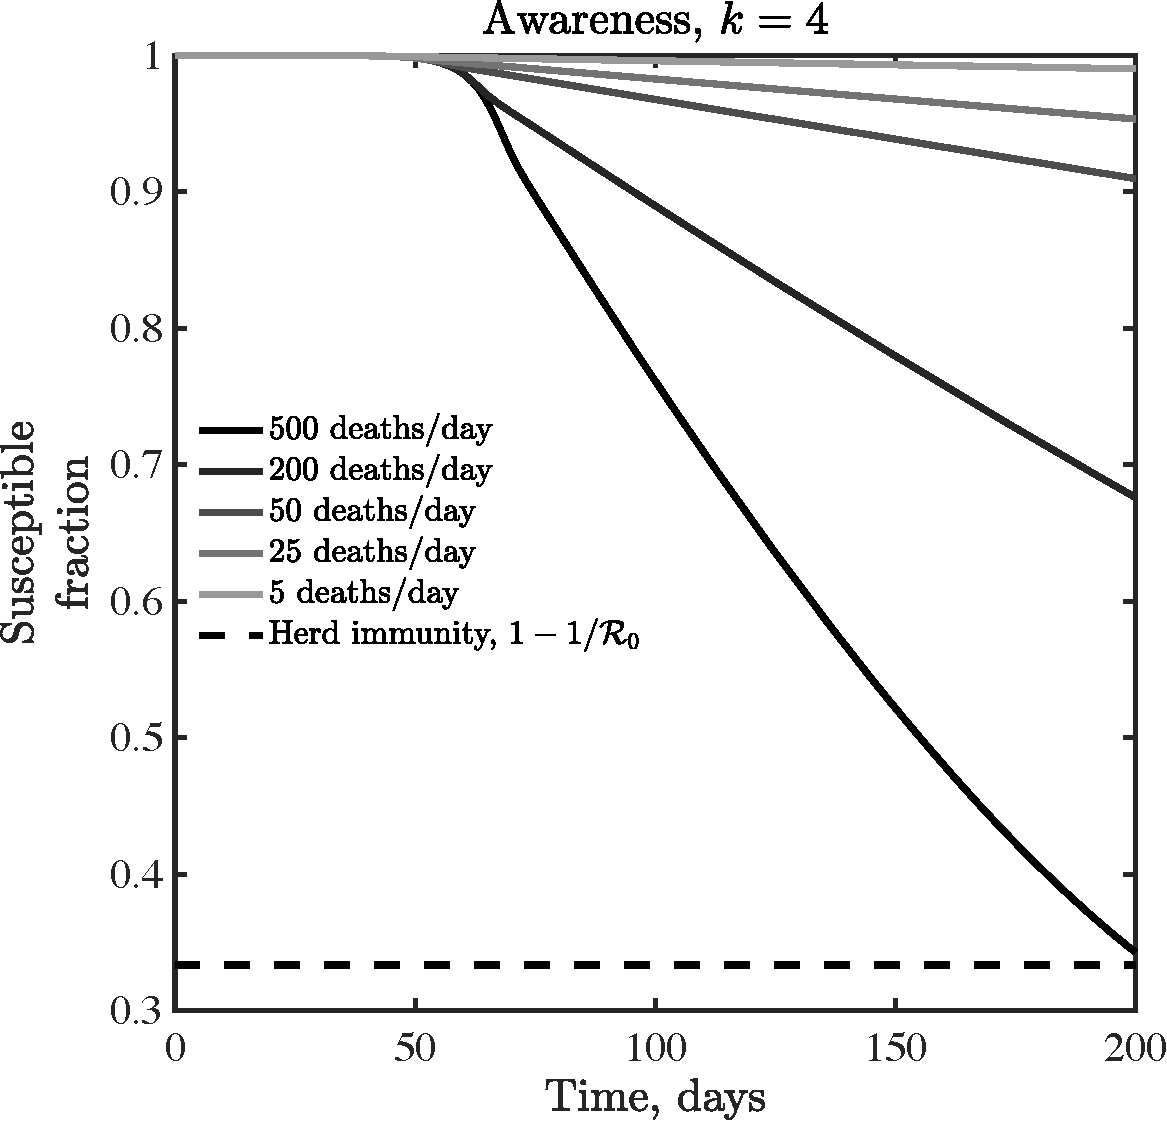
\includegraphics[width=0.4\textwidth]{scripts/figseir_Susc_k4_noname.pdf}
\caption{Dynamics given variation in the critical fatality awareness
level, $\delta_c$ for awareness $k=1$ (top) and $k=4$ (bottom). Panels show
deaths/day (top) and the susceptible fraction as a function of time (bottom),
the latter compared to a herd immunity
level when only a fraction $1/{\cal{R}}_0$ remain susecptible.
These simulations share the
epidemiological parameters 
$\beta=0.5$ /day, $\mu=1/2$ /day, $\gamma=1/6$ /day,
and $f_D=0.01$.
\label{fig.generic_k1-4}}
\end{center}
\end{figure*}

\begin{figure*}[t!]
\begin{center}
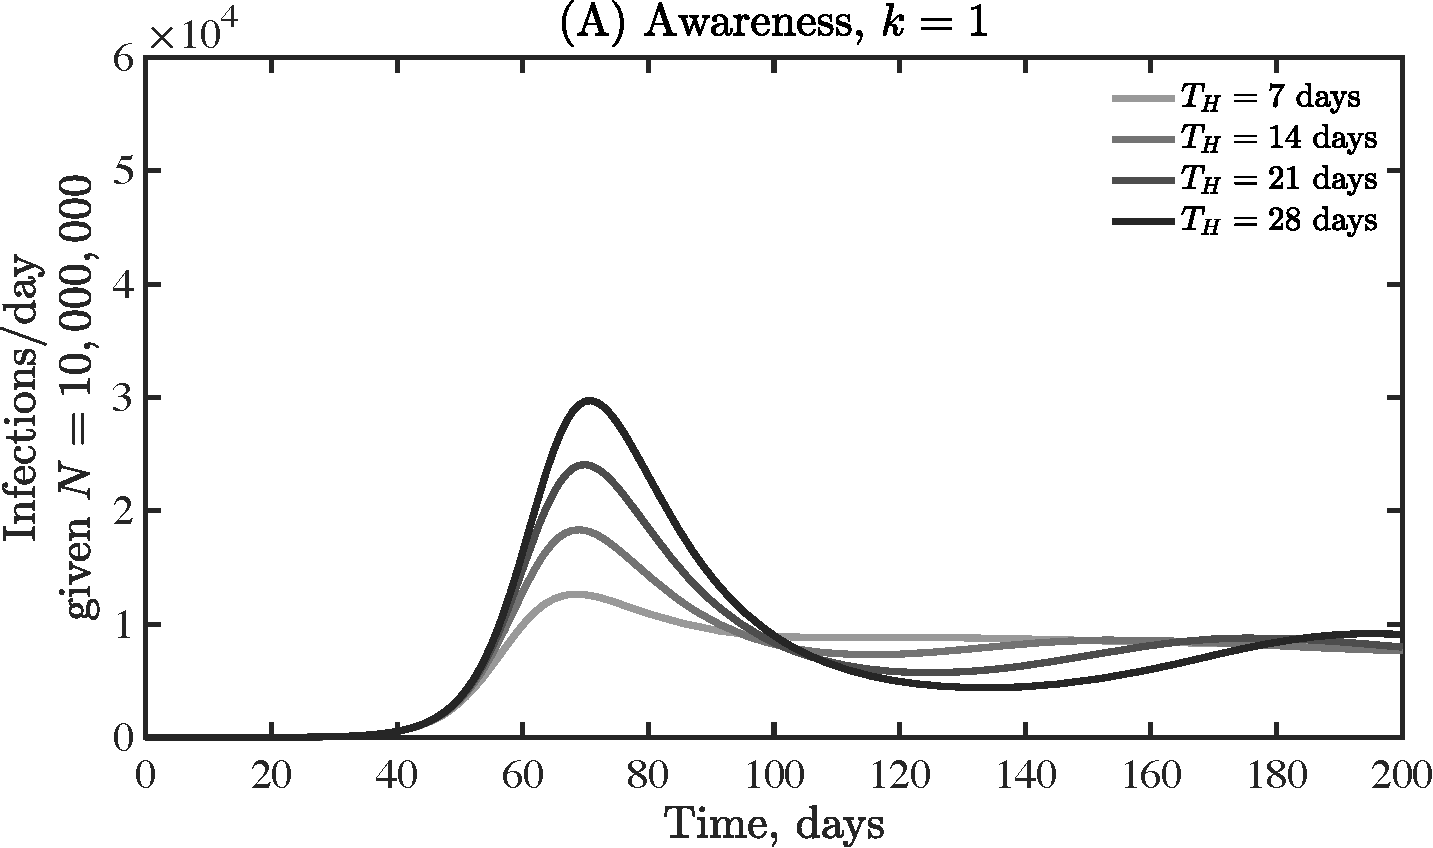
\includegraphics[width=0.4\textwidth]{scripts/figseir_Hdel_k1_noname.pdf}
\mbox{\hspace{0.05\textwidth}}
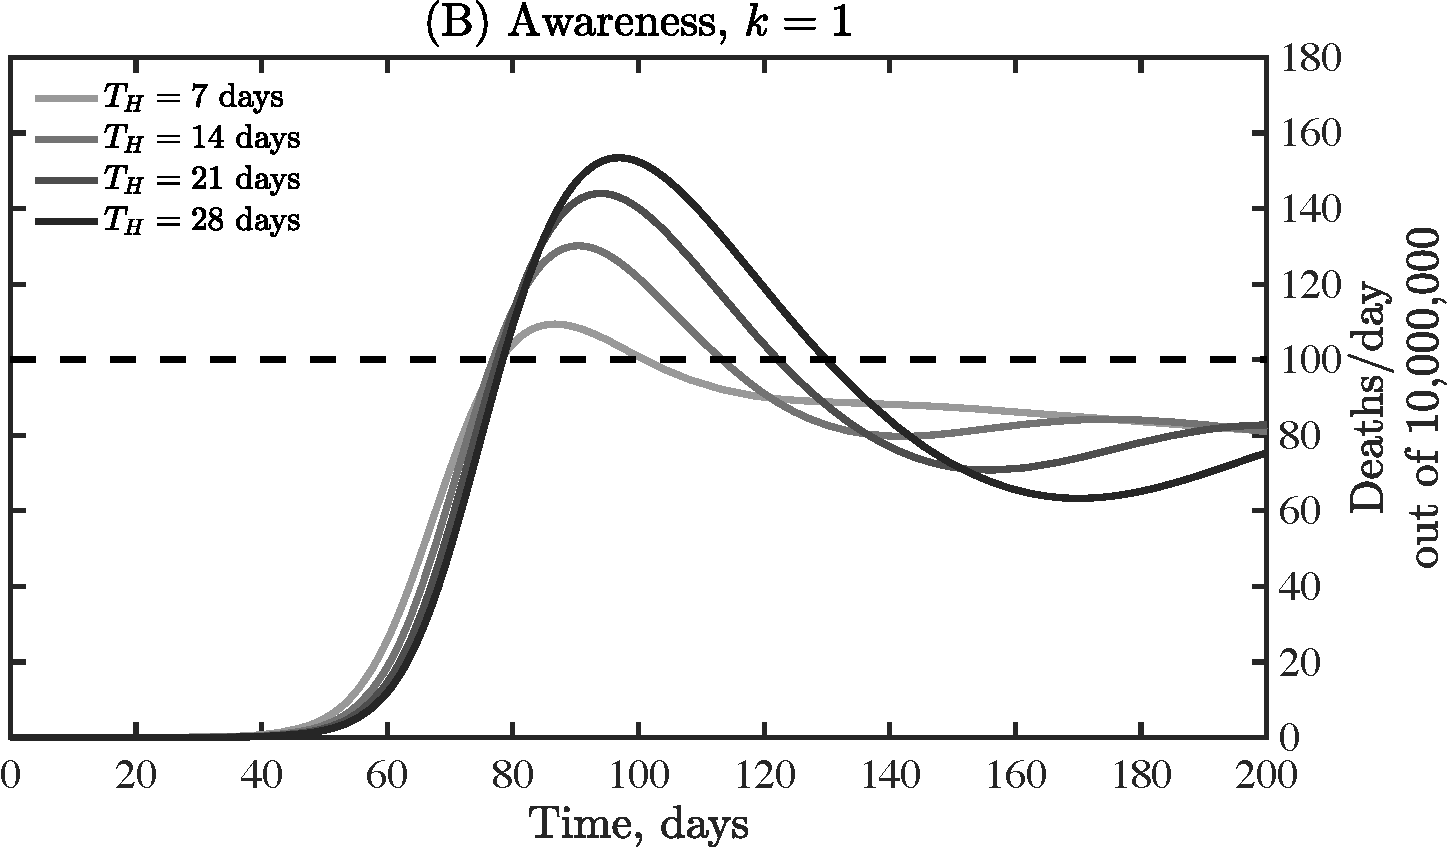
\includegraphics[width=0.4\textwidth]{scripts/figseir_Hdel_k1D_noname.pdf}\\
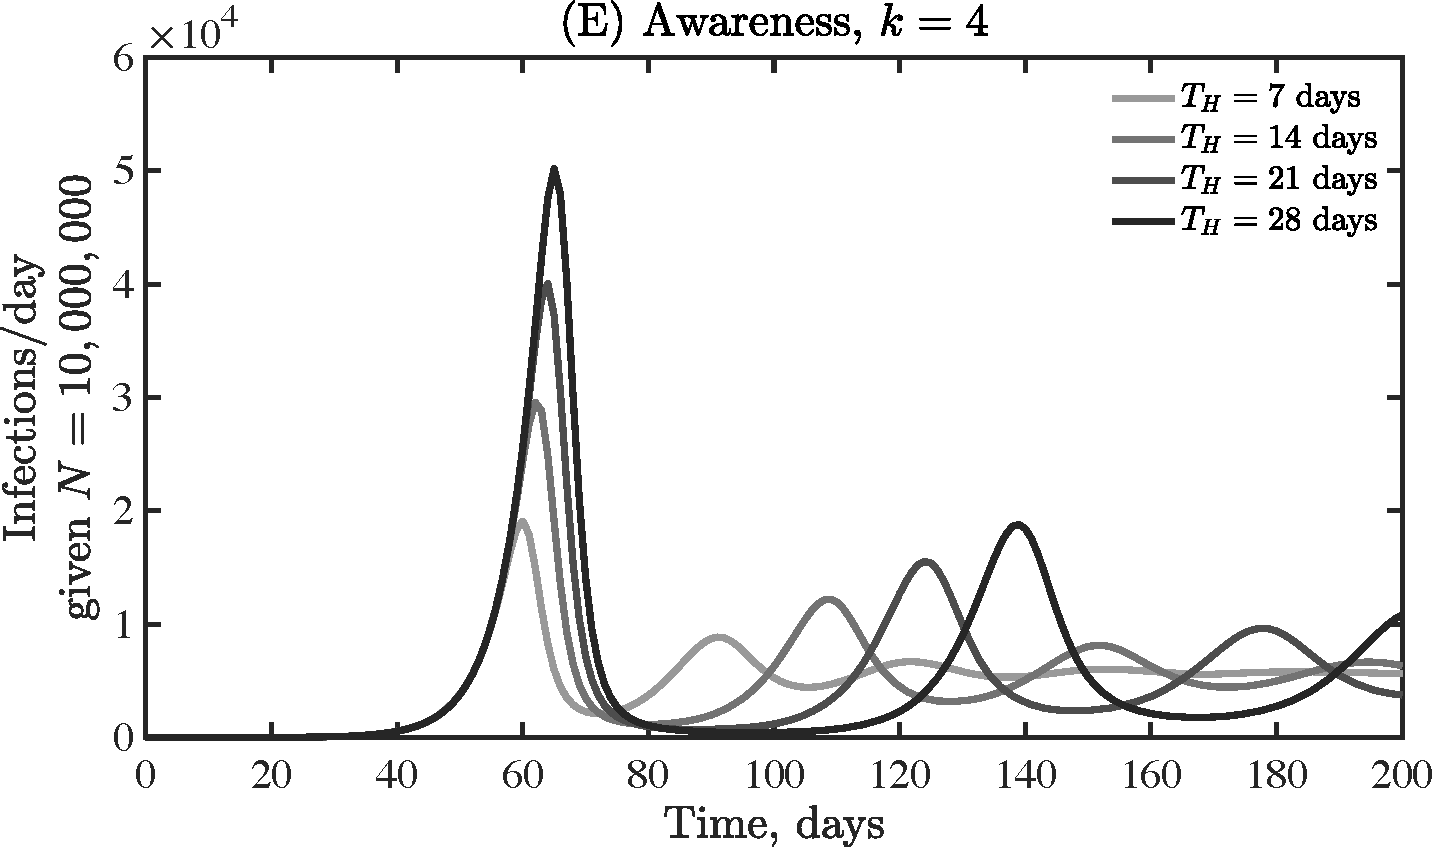
\includegraphics[width=0.4\textwidth]{scripts/figseir_Hdel_k4_noname.pdf}
\mbox{\hspace{0.05\textwidth}}
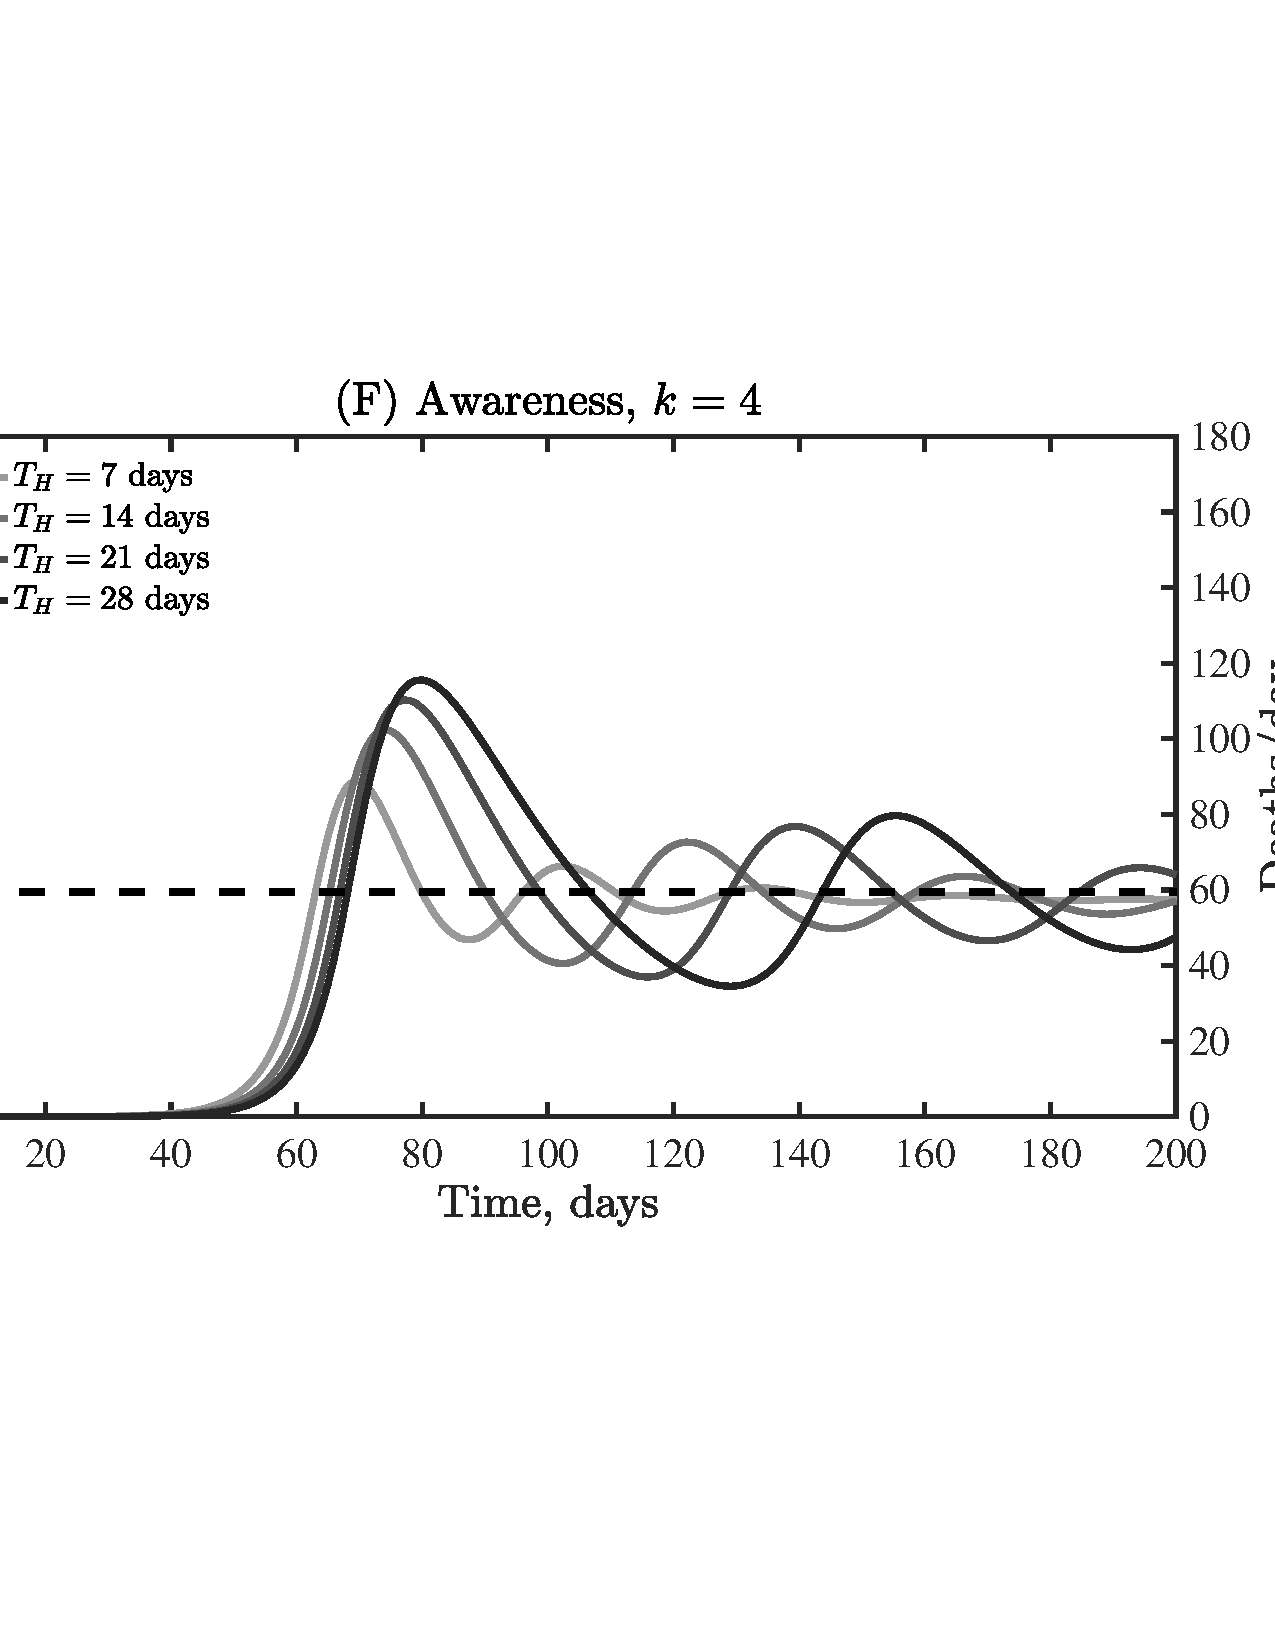
\includegraphics[width=0.4\textwidth]{scripts/figseir_Hdel_k4D_noname.pdf}
\caption{Emergence of oscillatory dynamics in a death-driven awareness
model of social distancing given lags between infection and fatality.
Awareness is $k=1$ (top) and $k=4$ (bottom), all other parameters as in Figure~\ref{fig.ID_day}.
The dashed
lines for fatalities expected quasi-stationary value $\delta^{(q)}$.
\label{fig.oscillate_k1-4}}
\end{center}
\end{figure*}

\begin{figure*}[t!]
\begin{center}
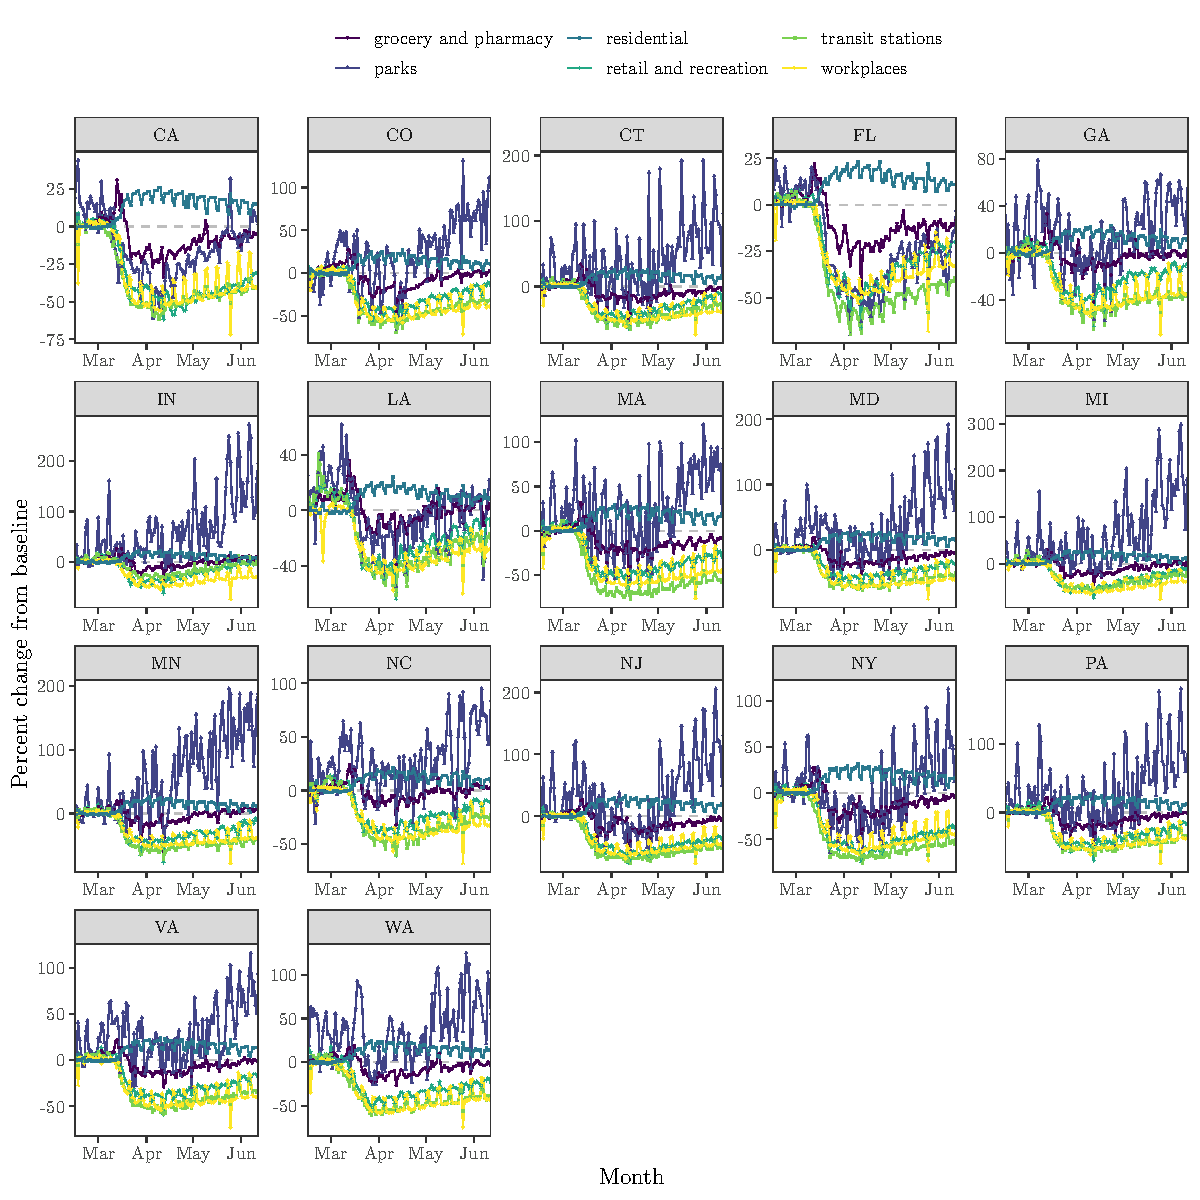
\includegraphics[width=0.95\textwidth]{deaths/mobility.pdf}
\caption{Percent mobility change from baseline across six categories in 17 states.
\label{fig.supp_mobility}}
\end{center}
\end{figure*}

